
Projekt ten powstał w technologii Windows Presentation Foundation. 
Jedną z metod rozdzielenia widoku od logiki biznesowej w interfejsie tworzonym w WPF jest wzorzec MVVM (ang. \textit{Model-View-ViewModel}). 
Jego cel to jasny podział aplikacji na \textit{Model} - dane naszej aplikacji, ich interakcja ze sobą i implementacja mechanizmów działania oprogramowania. 
\textit{View} odpowiada tylko za wyświetlanie danych użytkownikowi oraz przyjmowanie jego interakcji jak kliknięcia czy wprowadzanie informacji. 
Za to klasy \textit{ViewModel} zajmują sie na połączeniu modelu i widoku konwertując obiekty z części biznesowej na dane które mają dotrzeć do użytkownika. 
Ich zadaniem jest też obsługa danych wprowadzanych przez interfejs aplikacji.

\subsubsection{Model}

\begin{figure}[H]
    \centering
    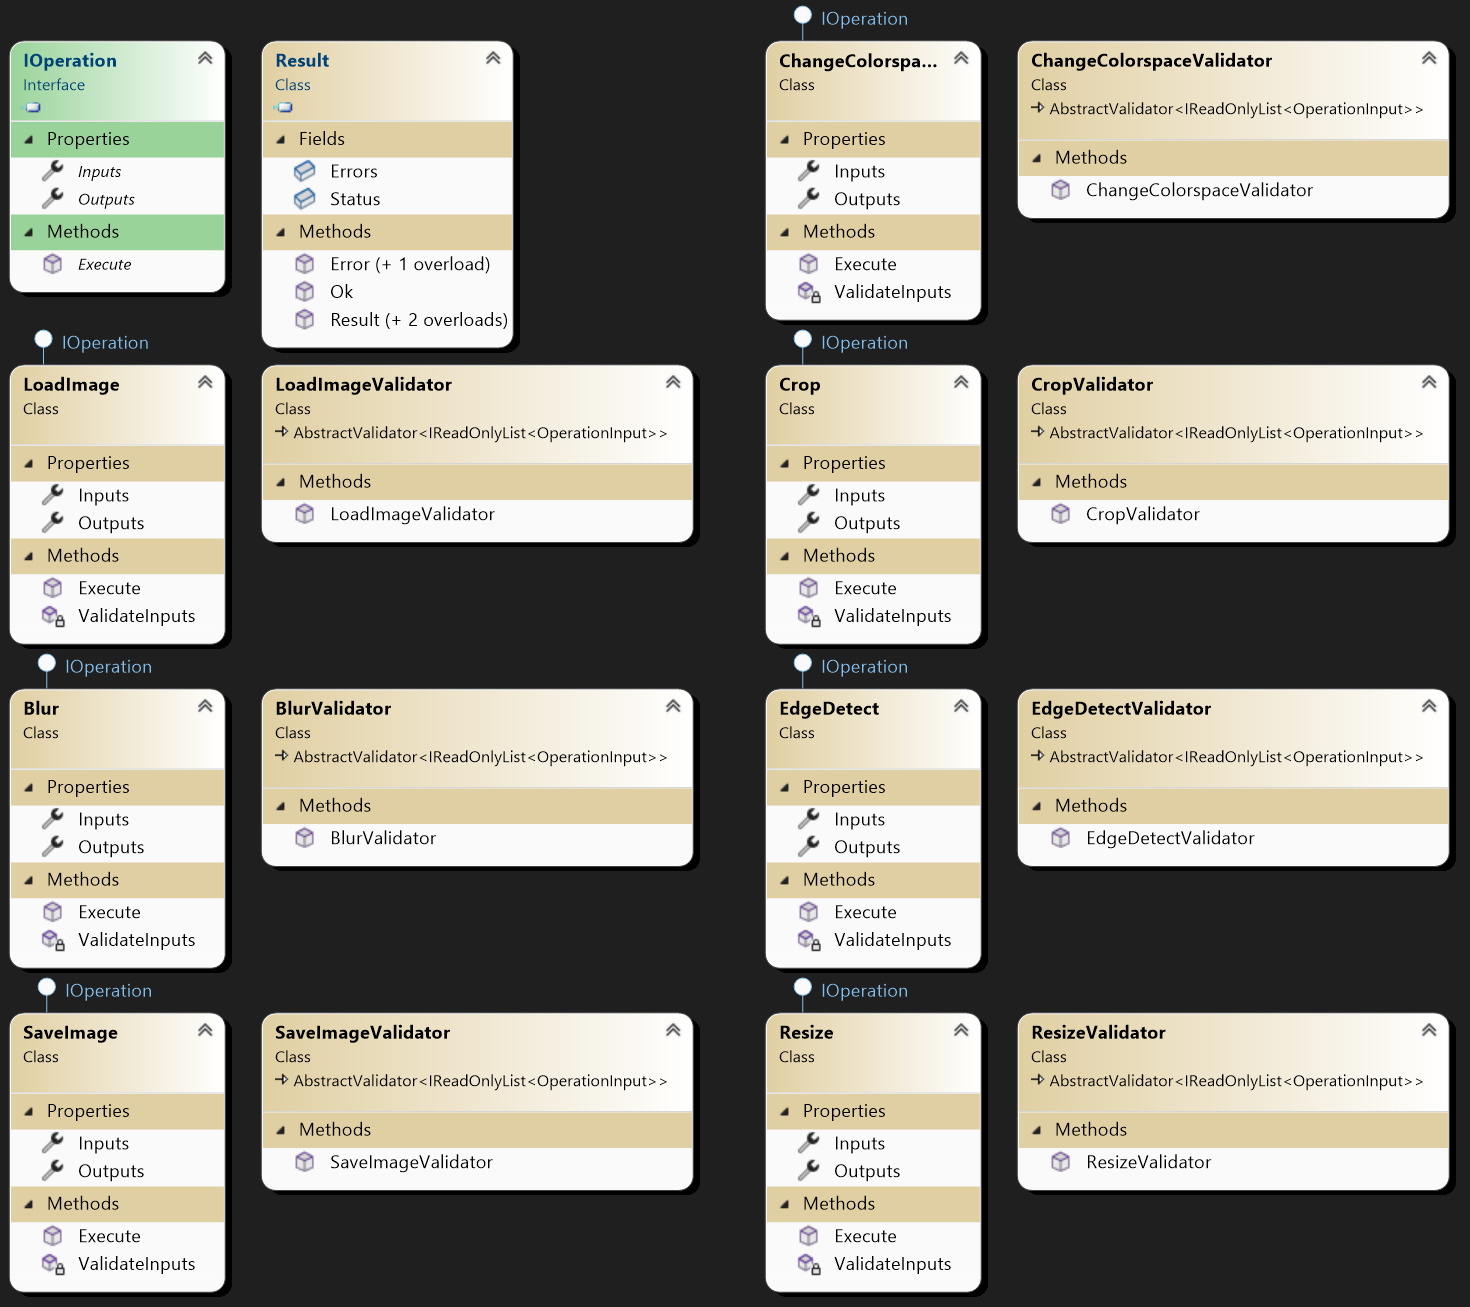
\includegraphics[width=1\linewidth]{images/Picture11.png}
    \caption{Diagram operacji. Opracowanie własne.}
    \label{fig:modelDiag}
\end{figure}

W NoodleCV warstwa \textit{Model} jest minimalna \autoref{fig:modelDiag}. 
Posiada interfejs IOperation odpowiadający za formę wszystkich implementacji operacji. 
Posiadają generyczna kolekcje wejść \textit{Inputs} oraz wyjść \textit{Outputs}.
Jedyna metoda zdefiniowana w nich to wykonanie operacji - zwraca ona obiekt \textit{Result}.
Informuje ona następne warstwy czy operacja się powiodła, jeżeli nie to dlaczego. 
Listę błędów otrzymujemy dzięki sprawdzeniu wejść za pomocą biblioteki Fluent Validation. 
Każda operacja wymaga swojego własnego walidatora danych i zapewnia tym bezpieczne działanie aplikacji - użytkownik nie powinien być w stanie doprowadzić programu do błędu złym parametrem operacji.

\begin{figure}[H]
    \centering
    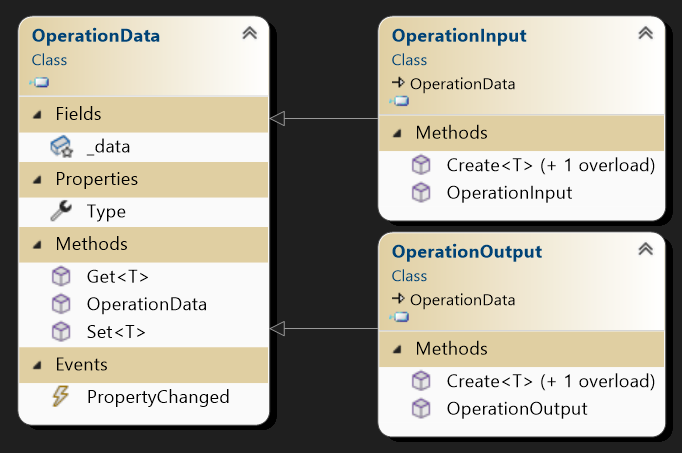
\includegraphics[width=0.6\linewidth]{images/Picture12.png}
    \caption{Diagram generycznych typów przechowujących dane operacji. Opracowanie własne.}
    \label{fig:input}
\end{figure}

Wejścia i wyjścia parametrów operacji mogą być w wielu różnych typach więc kolekcje przyjmujące te dane musiały być generyczne. 
Daje to dużo większą elastyczność ale może utrudnić implementację. 
Tworząc operacje i ich późniejsze \textit{ViewModel}'e trzeba zachować szczególną ostrożność. 
Przy tworzeniu nowych modeli zakładamy że obiekt w tym miejscu kolekcji będzie miał odpowiedni typ. 
Przy odczytywaniu danych z tej kolekcji nie ma informacji co to za klasa, należy poprawnie narzucić jej rodzaj inaczej napotkamy błąd i aplikacja wyłącza się.
Pomimo tych problemów warto korzystać z tej struktury ponieważ niektóre operacje przyjmują tylko ścieżkę do pliku w formie tekstu, inne mogą nie mieć żadnego wyjścia ale wszystkie pasują do jednego wspólnego interfejsu.

\subsubsection{View}



\subsubsection{ViewModel}
